\documentclass[tikz,border=6pt]{standalone}
\usepackage[T1]{fontenc}
\usepackage[utf8]{inputenc}
\usepackage{import}
\subimport{layers/}{init.tex}
\usetikzlibrary{arrows.meta,positioning}
\definecolor{ink}{HTML}{242629}
\definecolor{muted}{HTML}{59616a}
\definecolor{panel}{HTML}{f6f6f3}
\definecolor{blue}{HTML}{dfeaf5}
\definecolor{peach}{HTML}{f7cdae}
\definecolor{green}{HTML}{a9ce91}
\definecolor{yellow}{HTML}{ffe49b}
\definecolor{purple}{HTML}{d5c5e8}
\definecolor{white}{HTML}{ffffff}
\definecolor{heat}{HTML}{e89a50}
\definecolor{offset}{HTML}{a6bdd8}
\definecolor{size}{HTML}{ddc66e}
\definecolor{yaw}{HTML}{a8c983}
\definecolor{iou}{HTML}{b6a1cd}
\begin{document}
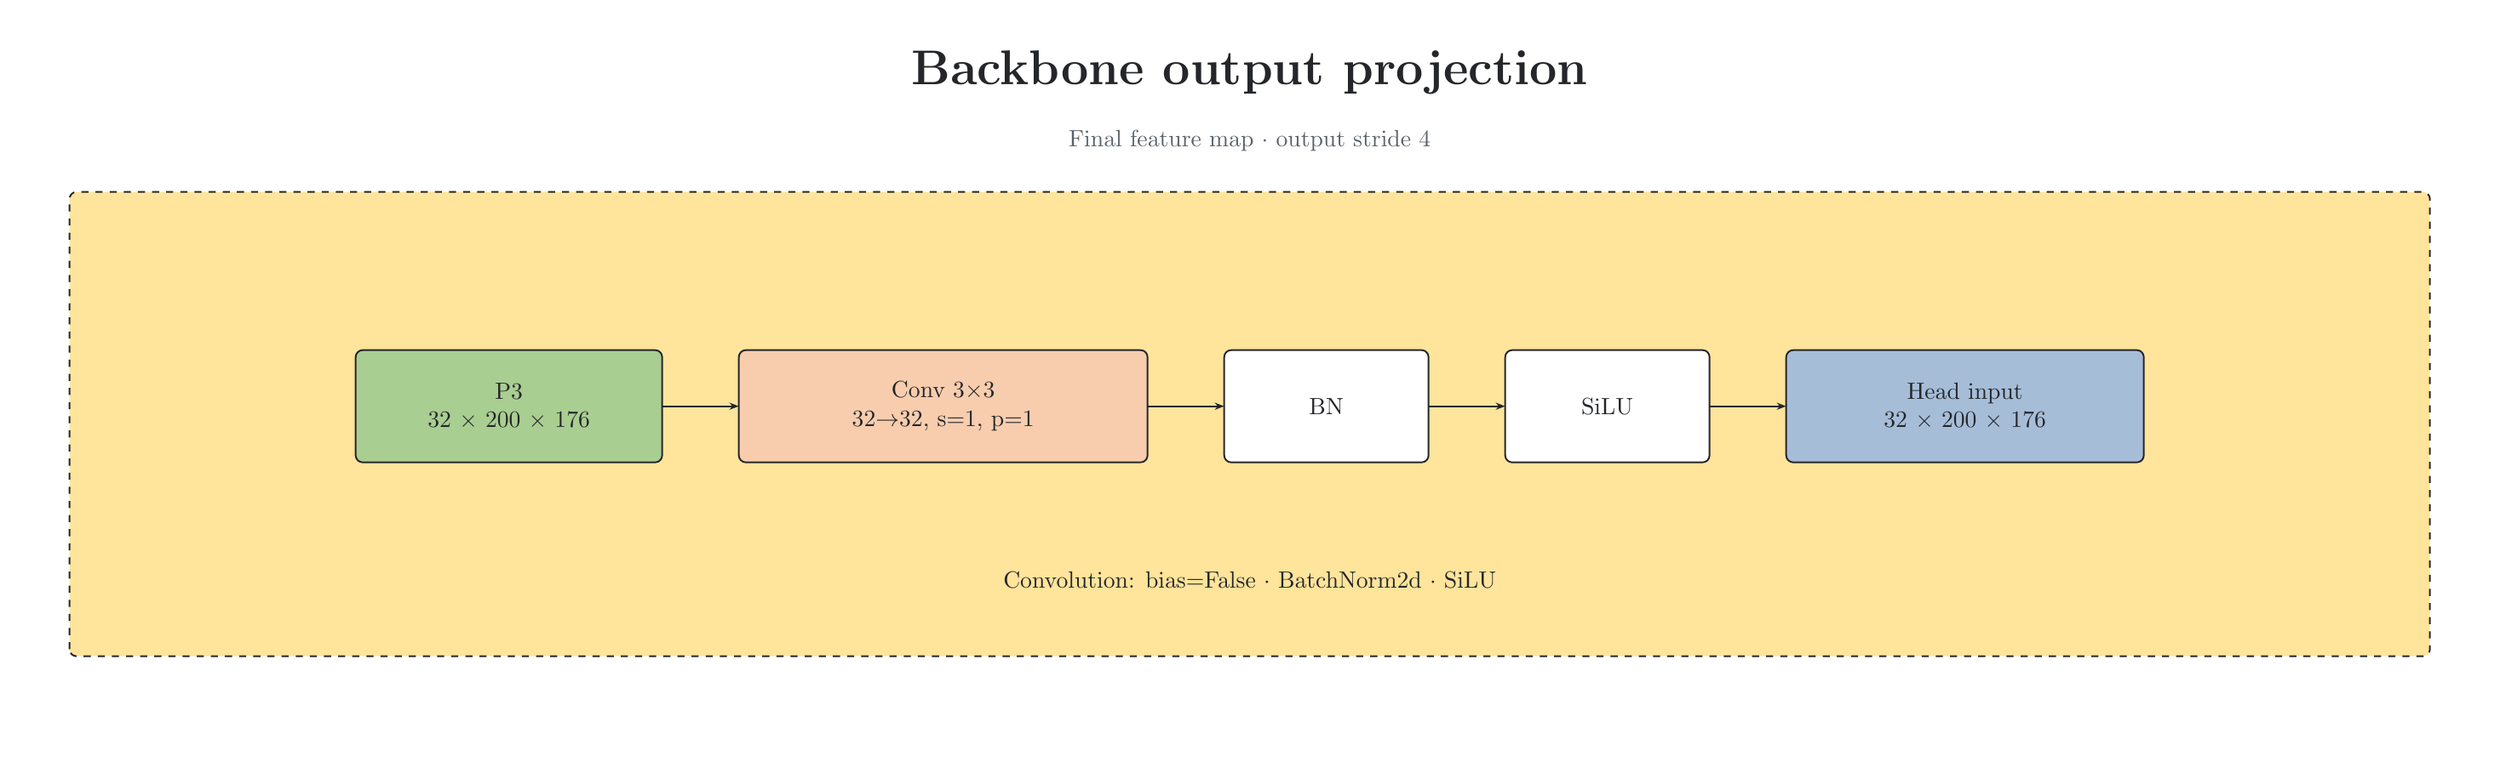
\begin{tikzpicture}[x=1.524cm,y=1.524cm,z={(0.9906cm,0.73152cm)}]
\path[use as bounding box] (0,0) rectangle (24,7);
\node[anchor=center,align=center,text=ink,font=\fontsize{20}{24.0}\selectfont \bfseries ] at (12.0,6.52) {Backbone output projection};
\node[anchor=center,align=center,text=muted,font=\fontsize{10}{12.0}\selectfont ] at (12.0,5.85) {Final feature map $\cdot$ output stride 4};
\draw[draw=ink,fill=yellow,rounded corners=3pt,line width=.7pt,dashed] (0.4499999999999993,0.8000000000000003) rectangle (23.55,5.35);
\node[anchor=west,align=left,text=ink,font=\fontsize{15}{18.0}\selectfont \bfseries ] at (0.8,4.85) {};
\draw[draw=ink,fill=green,rounded corners=3pt,line width=.7pt] (3.25,2.7) rectangle (6.25,3.8);
\node[anchor=center,align=center,text=ink,font=\fontsize{10}{12.0}\selectfont ] at (4.75,3.25) {P3\\32 $\times$ 200 $\times$ 176};
\draw[-{Stealth[length=4pt]},draw=ink,line width=.7pt] (6.25,3.25) -- (7.0,3.25);
\draw[draw=ink,fill=peach,rounded corners=3pt,line width=.7pt] (7.0,2.7) rectangle (11.0,3.8);
\node[anchor=center,align=center,text=ink,font=\fontsize{10}{12.0}\selectfont ] at (9.0,3.25) {Conv 3$\times$3\\32$\rightarrow$32, s=1, p=1};
\draw[-{Stealth[length=4pt]},draw=ink,line width=.7pt] (11.0,3.25) -- (11.75,3.25);
\draw[draw=ink,fill=white,rounded corners=3pt,line width=.7pt] (11.75,2.7) rectangle (13.75,3.8);
\node[anchor=center,align=center,text=ink,font=\fontsize{10}{12.0}\selectfont ] at (12.75,3.25) {BN};
\draw[-{Stealth[length=4pt]},draw=ink,line width=.7pt] (13.75,3.25) -- (14.5,3.25);
\draw[draw=ink,fill=white,rounded corners=3pt,line width=.7pt] (14.5,2.7) rectangle (16.5,3.8);
\node[anchor=center,align=center,text=ink,font=\fontsize{10}{12.0}\selectfont ] at (15.5,3.25) {SiLU};
\draw[-{Stealth[length=4pt]},draw=ink,line width=.7pt] (16.5,3.25) -- (17.25,3.25);
\draw[draw=ink,fill=offset,rounded corners=3pt,line width=.7pt] (17.25,2.7) rectangle (20.75,3.8);
\node[anchor=center,align=center,text=ink,font=\fontsize{10}{12.0}\selectfont ] at (19.0,3.25) {Head input\\32 $\times$ 200 $\times$ 176};
\node[anchor=center,align=center,text=ink,font=\fontsize{10}{12.0}\selectfont ] at (12.0,1.55) {Convolution: bias=False $\cdot$ BatchNorm2d $\cdot$ SiLU};
\end{tikzpicture}
\end{document}
